\chapter{Deep Reinforcement Learning (DRL)}\label{Deep Reinforcement Learning (DRL)}

\section*{Intro \cite{drl-1}}

\begin{table}[H]
    \begin{minipage}{0.45\linewidth}
        \begin{figure}[H]
            \centering
            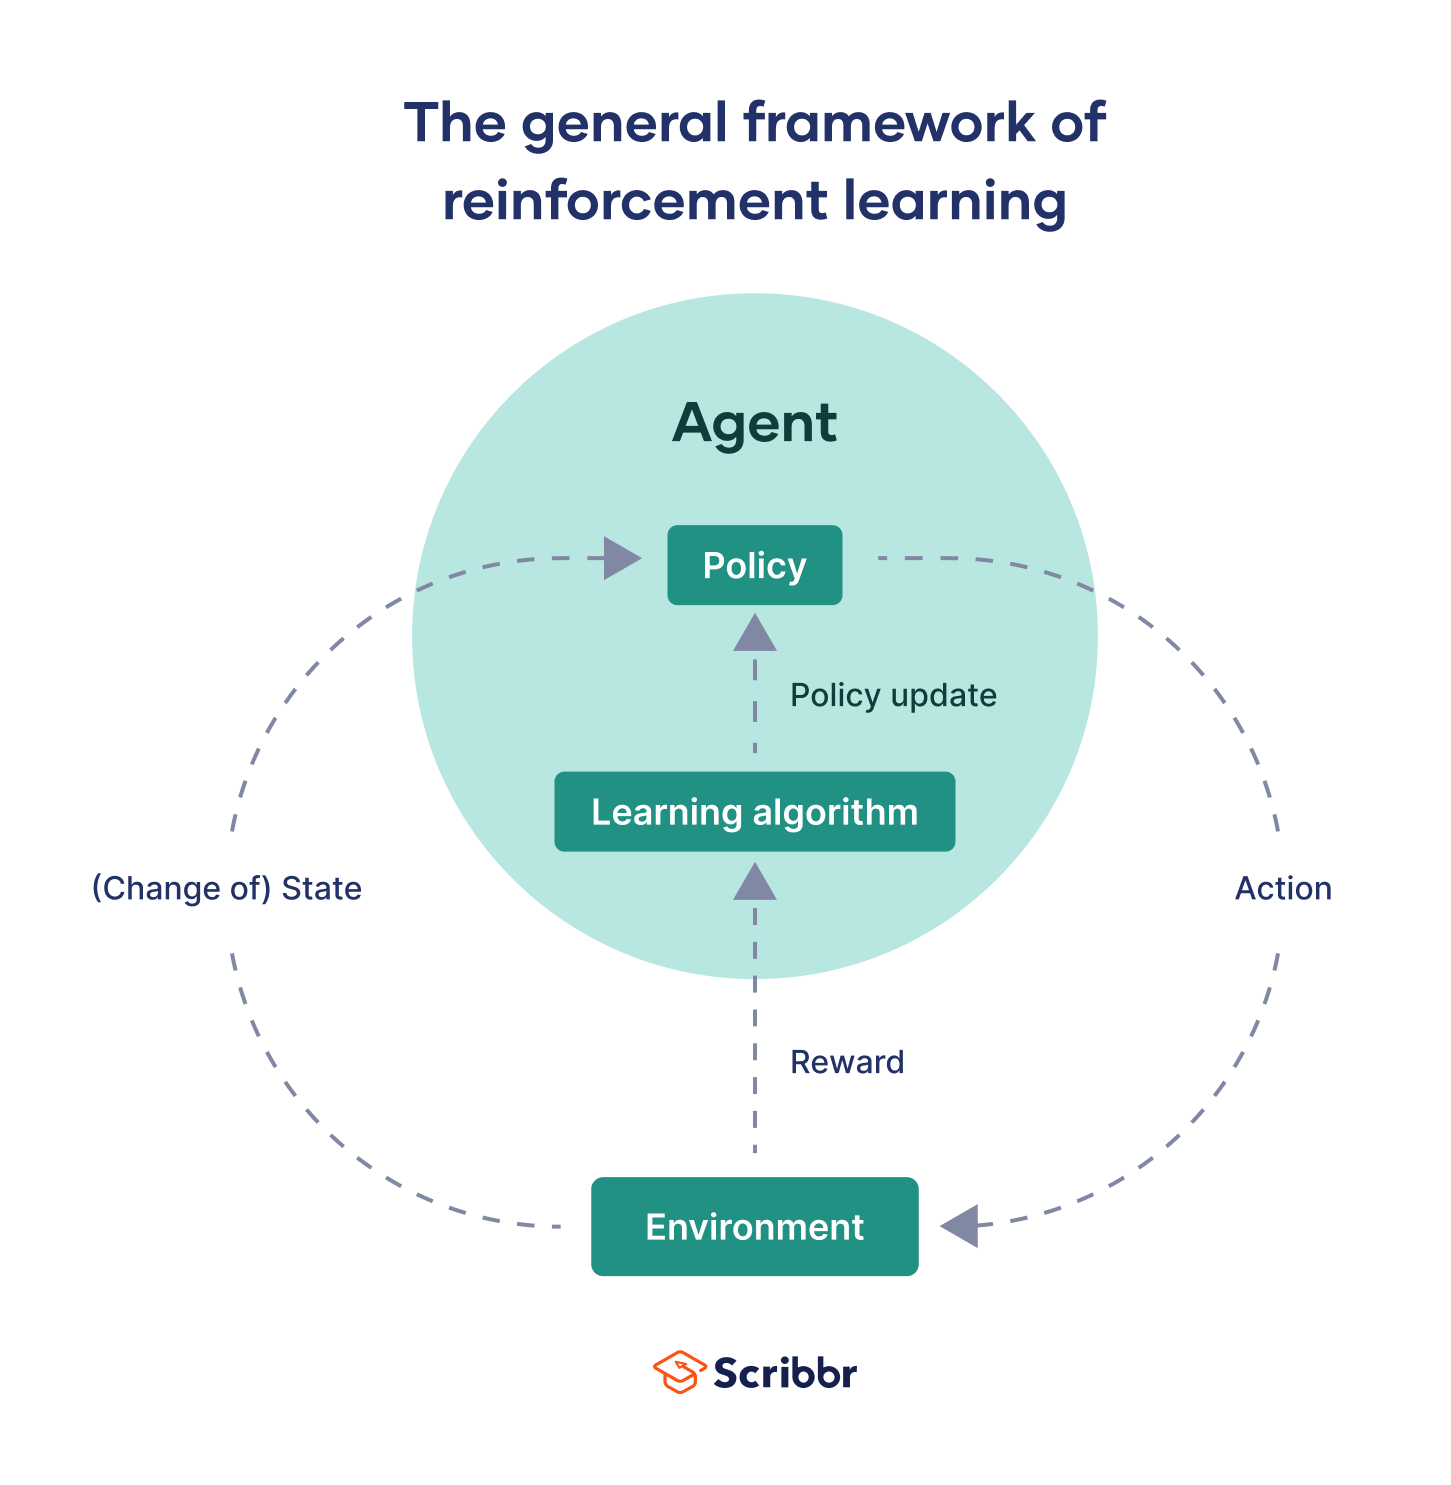
\includegraphics[height=7cm]{Pictures/deep-reinforcement-learning/drl-flow.jpg}
            \caption{Deep Reinforcement Learning}
        \end{figure}        
    \end{minipage}
    \hfill
    \begin{minipage}{0.45\linewidth}
        “\textbf{Reinforcement learning}” to refer to decision-making with uncertain models, and in addition, current actions alter the future behavior of the system. Therefore, if the same action is taken at a future time, the consequences might not be the same. This additional feature distinguishes RL from “mere” decision-making under uncertainty.\cite{arxiv-2304.00803}
    \end{minipage}
\end{table}








































